 %%%%%%%%%%%%%%%%%%%%%%%%%%%%%%%%%%%%%%%%%% 
 % @File    : c:\Users\Administrator\Desktop\白板学习笔记\数学部分\RL_math.tex
 % @Date    : 2021-01-25 21:49:30
 % @Author  : RankFan
 % @Email   : 1917703489@qq.com
 % -----
 % Last Modified: 2021-02-07 16:55:03
 % Modified By: Rank_fan
 % -----
 %%%%%%%%%%%%%%%%%%%%%%%%%%%%%%%%%%%%%%%%%% 

 %%============================宏包=======================================%
\documentclass[11pt]{article}
\usepackage{ctex}
%\usepackage[left=1.25in,right=1.25in,top=1in,bottom=1in]{geometry}
% Copyright 20120 Liutao Tian, MIT License
% https://github.com/andy123t/code-latex-style/

\usepackage{listings,xcolor}

% Matlab highlight color settings
%\definecolor{mBasic}{RGB}{248,248,242}       % default
\definecolor{mKeyword}{RGB}{0,0,255}          % bule
\definecolor{mString}{RGB}{160,32,240}        % purple
\definecolor{mComment}{RGB}{34,139,34}        % green
\definecolor{mBackground}{RGB}{245,245,245}   % lightgrey
\definecolor{mNumber}{RGB}{128,128,128}       % gray

% Matlab highlight color settings
%\definecolor{mBasic}{RGB}{248,248,242}       % default
\definecolor{mKeyword}{RGB}{0,0,255}          % bule
\definecolor{mString}{RGB}{160,32,240}        % purple
\definecolor{mComment}{RGB}{34,139,34}        % green
\definecolor{mBackground}{RGB}{245,245,245}   % lightgrey
%\definecolor{mNumber}{RGB}{128,128,128}       % gray
\definecolor{mNumber}{RGB}{134,145,148}       % gray
\definecolor{mNumberbg}{RGB}{237,240,241}     % lightgrey

% Python highlight color settings
%\definecolor{pBasic}{RGB}{248, 248, 242}     % default
\definecolor{pKeyword}{RGB}{228,0,128}        % magenta
\definecolor{pString}{RGB}{148,0,209}         % purple
\definecolor{pComment}{RGB}{117,113,94}       % gray
\definecolor{pIdentifier}{RGB}{166, 226, 46}  %
\definecolor{pBackground}{RGB}{245,245,245}   % lightgrey
\definecolor{pNumber}{RGB}{128,128,128}       % gray

\lstnewenvironment{Matlab}[1]{
\lstset{language=Matlab,               % choose the language of the code
  %frame=tlbr,
  xleftmargin=10pt,
  xrightmargin=10pt,
  frame=l,
  framesep=15pt,%framerule=0pt,  % sets the frame style
  %frame=shadowbox,rulesepcolor=\color{red!20!green!20!blue!20},
  basicstyle=\small\ttfamily,
  keywordstyle={\color{mKeyword}},     % sets color for keywords
  stringstyle={\color{mString}},       % sets color for strings
  commentstyle={\color{mComment}},     % sets color for comments
  backgroundcolor=\color{mBackground}, % choose the background color
  title=#1,                            % \lstname show the filename of files
  keywords={break,case,catch,classdef,continue,else,elseif,end,for,
  function,global,if,otherwise,parfor,persistent,return,spmd,switch,try,while},
  showspaces=false,                    % show spaces adding particular underscores
  showstringspaces=false,              % underline spaces within strings
  showtabs=false,                      % show tabs within strings adding particular underscores
  tabsize=4,                           % sets default tabsize to 2 spaces
  captionpos=t,                        % sets the caption-position to bottom
  breaklines=true,                     % sets automatic line breaking
  framexleftmargin=5pt,
  fillcolor=\color{mNumberbg},
  rulecolor=\color{mNumberbg},
  numberstyle=\tiny\color{mNumber},
  numbersep=9pt,                      % how far the line-numbers are from the code
  numbers=left,                        % where to put the line-numbers
  stepnumber=1,                        % the step between two line-numbers.
}}{\lstname}

\lstnewenvironment{Python}[1]{
\lstset{language=python,               % choose the language of the code
  xleftmargin=10pt,
  xrightmargin=10pt,
  frame=l,
  framesep=15pt,%framerule=0pt,  % sets the frame style
  %frame=shadowbox,rulesepcolor=\color{red!20!green!20!blue!20},
  %basicstyle=\small\ttfamily,          % sets font style for the code
  basicstyle=\footnotesize\fontspec{Consolas},
  keywordstyle=\color{pKeyword},       % sets color for keywords
  stringstyle=\color{pString},         % sets color for strings
  commentstyle=\color{pComment},       % sets color for comments
  backgroundcolor=\color{pBackground}, % choose the background color
  title=#1,                            %\lstname show the filename of files
  emph={format_string,eff_ana_bf,permute,eff_ana_btr},
  emphstyle=\color{pIdentifier}
  showspaces=false,                    % show spaces adding particular underscores
  showstringspaces=false,              % underline spaces within strings
  showtabs=false,                      % show tabs within strings adding particular underscores
  tabsize=4,                           % sets default tabsize to 2 spaces
  captionpos=t,                        % sets the caption-position to bottom
  breaklines=true,                     % sets automatic line breaking
  framexleftmargin=5pt,
  fillcolor=\color{mNumberbg},
  rulecolor=\color{mNumberbg},
  numberstyle=\tiny\color{mNumber},
  numbersep=9pt,                      % how far the line-numbers are from the code
  numbers=left,                        % where to put the line-numbers
  stepnumber=1,                        % the step between two line-numbers.
}}{}



 \usepackage{amsmath}
 \usepackage{booktabs}
 \usepackage{amsthm}
 \usepackage{graphicx}
 \usepackage{amssymb}
 \usepackage{authblk}
 
 \usepackage{tikz}  % tikz
 \usepackage[left=2cm,right=2cm,top=2.5cm,bottom=3cm]{geometry} % 页面设置
 \usepackage[bookmarks, bookmarksnumbered ,colorlinks, linkcolor = blue, citecolor = myred ]{hyperref} %超链接
 %\usepackage{fontspec}  % for Consolas
 \definecolor{myred}{rgb}{153, 0, 0}

 \tikzset{>=stealth}
 \usetikzlibrary{arrows,shapes,positioning,matrix}

 %%============================NewComman=======================================%
 \newcommand*{\email}[1]{%
    \normalsize\href{mailto:#1}{#1}\par
    }
\newcommand{\tikzmark}[3][]
    {\tikz[remember picture, baseline]
      \node [anchor=base,#1](#2) {#3};
      }
%%============================定理环境=======================================%
\newtheorem{mydef}{Definition}[section]
\newtheorem{myproof}{Proof}[section]
\newtheorem{myexample}{Example}[section]
%%============================命令更新=======================================%
\renewcommand \Authands{ \&  } 

%%============================计数器设置=======================================%
 \numberwithin{equation}{section}
 \numberwithin{figure}{section}
 \graphicspath{{figures/}}

 %%================================== 设置中文字体 ================================%
\xeCJKsetup{AutoFakeBold=true}
\setCJKmainfont{FZShuSong-Z01}[BoldFont={FZHei-B01},ItalicFont={FZKai-Z03}]
\setCJKsansfont{FZHei-B01}
\setCJKmonofont{FZShuSong-Z01}
%================================== 设置英文字体 ================================%TeX Gyre Pagella
\setmainfont[Mapping=tex-text]{Times New Roman}%--------------------------------英文衬线字体
% \setmainfont{TeX Gyre Pagella}


 \title{机器学习--数学部分}
 \author[1]{RankFan \thanks{fanxiaolong98@gmail.com}}
 \author[2]{JIE \thanks{fanxiaolong98@gmail.com}}
 \affil[1] {公众号:经济知识综合 }
 \affil[2] {公众号:经济知识综合 }

\begin{document}
\maketitle
\newpage
\tableofcontents
\newpage
 %%%%%%%%%%%%%%%%%%%%%%%%%%%%%%%%%%%%%%%%%% 
 % @File    : c:\Users\Administrator\Desktop\白板学习笔记\数学部分\RL_math.tex
 % @Date    : 2021-01-25 21:49:30
 % @Author  : RankFan
 % @Email   : 1917703489@qq.com
 % -----
 % Last Modified: 2021-02-28 18:43:38
 % Modified By: RankXiaoLong
 % -----
 %%%%%%%%%%%%%%%%%%%%%%%%%%%%%%%%%%%%%%%%%% 

 %%============================宏包=======================================%
 \section{多维高斯分布}
 $ \boldsymbol{x} \in \mathbb{R}^{p} $ , $ \boldsymbol{x} $ 是一个随机变量。
\[  \boldsymbol{x} \sim N(\mu,\Omega) \]
\[ p(\boldsymbol{x})= \frac{1}{{2 \pi}^{\frac{p}{2}} \left| \Omega \right|^{\frac{1}{2}}  } 
        exp\{  -\frac{1}{2} {\left( \boldsymbol{x - \mu}  \right)}^{T} \boldsymbol{\Omega^{-1}} \left( \boldsymbol{x - \mu}  \right)\} \]  
        
 $\boldsymbol{\Omega} $是正定阵,一般是半正定阵.通常而言是半正定的对称阵。
\[       \boldsymbol{x} =  \begin{pmatrix}
            x_1 \\
            x_2 \\
            \vdots\\
            x_p
        \end{pmatrix} \quad 
        \boldsymbol{\mu } =  \begin{pmatrix}
            \mu_1 \\
            \mu_2 \\
            \vdots\\
            \mu_p
        \end{pmatrix} \quad
        \boldsymbol{\Omega} =   \begin{pmatrix}
            \sigma_{11} & \sigma_{12} & \cdots & \sigma_{1p} \\
            \sigma_{21} & \sigma_{22} & \cdots & \sigma_{2p}\\
            \vdots&\vdots&  \ddots &\vdots \\\
            \sigma_{p1} & \sigma_{p2} & \cdots & \sigma_{pp}
           \end{pmatrix} \] 

  $  {\left( \boldsymbol{x - \mu}  \right)}^{\prime} \boldsymbol{\Omega^{-1}} \left( \boldsymbol{x - \mu}  \right) $  可以看做是一个关于
  $ \boldsymbol{x} , \boldsymbol{\mu}$ 之间的一个马氏距离。 $ \boldsymbol{\Sigma} = \boldsymbol{\Omega}^{-1} $ 为精度矩阵。

  \subsection{马氏距离}
  \begin{myexample}[马氏距离的定义]
    \[ \boldsymbol{z_1} = 
    \begin{pmatrix}
        z_{11} \\
        z_{12}
    \end{pmatrix} \quad 
    \boldsymbol{z_2} = 
    \begin{pmatrix}
        z_{21} \\
        z_{22}
    \end{pmatrix} \]
    \[
        \boldsymbol{(z_{1} -z_{2})}^{T} \Omega^{-1} \boldsymbol{(z_{1} -z_{2})} = 
        \left( z_{11}- z_{21}, z_{12}- z_{22}\right)  \boldsymbol{\Omega^{-1}} 
        \begin{pmatrix}
            z_{11}- z_{21} \\
            z_{12}- z_{22}
        \end{pmatrix} \]
        
        马氏距离与欧式距离的联系:$ \boldsymbol{\Omega = I} $时,马氏距离 = 欧式距离。
  \end{myexample}
  \begin{mydef}[方差矩阵]
    \[ \boldsymbol{\Omega  = U \Lambda U^{T} } \]

    $ \boldsymbol{\Omega} $是对称正定阵,可进行矩阵分解。$ diag(\lambda_{i}) $是对角矩阵。$ \boldsymbol{\Omega} $可以对称正交化。
  \begin{align*}
    \boldsymbol{ UU^{T}}  & = ~ \boldsymbol{U^{T} U   = I} \\
    \boldsymbol{\Lambda} & = ~ diag(\lambda_{i} ) \quad i = 1 , 2 ,\ldots ,p\\
    \boldsymbol{U} & = ~ \boldsymbol{( u_1,u_2,\cdots, u_p)}; \quad 
    \boldsymbol{u_i} ~~ is ~~ a  ~~ column ~~ vector (p \times 1),\| \boldsymbol{u_i} \| = 1 \\
    \Longrightarrow \qquad \boldsymbol{\Omega}  & = ( \boldsymbol{u_1,u_2,\cdots, u_p})  
    \begin{pmatrix}
        \lambda_{1} &  &  &  \\
        & \lambda_{2} & & \\
        & &  \ddots & \\\
        &  &  & \lambda_{p}
       \end{pmatrix}   
       \begin{pmatrix}
        \boldsymbol{u_1^{T}} \\
        \boldsymbol{u_2^{T}} \\
        \vdots\\
        \boldsymbol{u_p^{T}}
    \end{pmatrix} \\
    & = ( \boldsymbol{u_1} \lambda_{1} ,\boldsymbol{u_2} \lambda_{2} ,\cdots, \boldsymbol{u_p} \lambda_{p} ) 
     \begin{pmatrix}
        \boldsymbol{u_1^{T}} \\
        \boldsymbol{u_2^{T}} \\
        \vdots\\
        \boldsymbol{u_p^{T}}
     \end{pmatrix}  = \sum_{i = 1}^{p} \boldsymbol{u_{i}} \lambda_{i} \boldsymbol{u_{i}^{T}}
  \end{align*}
\end{mydef}
  \begin{align*}      
    \Longrightarrow \qquad \boldsymbol{\Omega^{-1}}  & = \boldsymbol{ \left( U \Lambda U^{T} \right) }^{-1} = \boldsymbol{U \Lambda^{-1} U^{T}} \\ 
    \boldsymbol{\Lambda^{-1}} &  = ~ diag(\lambda_{i}^{-1}) \quad i = 1 , 2 ,\ldots ,p \\
    \boldsymbol{\Omega^{-1}} &  = \sum_{i = 1}^{p} \boldsymbol{u_{i}} \lambda_{i}^{-1} \boldsymbol{u_{i}^{T}}  \\
    \Longrightarrow \qquad 
    {\left( \boldsymbol{x - \mu}  \right)}^{T} \boldsymbol{\Omega^{-1}} \left( \boldsymbol{x - \mu}  \right) 
    & =  {\left( \boldsymbol{x - \mu}  \right)}^{T}  \sum_{i = 1}^{p} \boldsymbol{u_{i}} \lambda_{i}^{-1} \boldsymbol{u_{i}^{T}}  
      \left( \boldsymbol{x - \mu}  \right) \\
    & =  \sum_{i = 1}^{p} {\left( \boldsymbol{x - \mu}  \right)}^{T}   \boldsymbol{u_{i}} \lambda_{i}^{-1} \boldsymbol{u_{i}^{T}} \left( \boldsymbol{x - \mu}  \right)  
  \end{align*}

  令$ y_{i} = {\left( \boldsymbol{x - \mu}  \right)}^{T}   \boldsymbol{u_{i}}$ ,  $ y_{i} $ 是一个标量, 几何意义是
  $ {\left( \boldsymbol{x - \mu}  \right)}^{T} $ 在 $ \boldsymbol{u_{i}}$ 上的投影。
$  \boldsymbol{y} = \begin{pmatrix}
        y_1 \\
        y_2 \\
        \vdots\\
        y_p
    \end{pmatrix}$
\[ \Longrightarrow \qquad {\left( \boldsymbol{x - \mu}  \right)}^{T} \boldsymbol{\Omega^{-1}} \left( \boldsymbol{x - \mu}  \right) 
              =   \sum_{i = 1}^{p} y_{i} {\lambda_{i}}^{-1} y_{i}  = \sum_{i = 1}^{p} y_{i}^{2} {\lambda_{i}}^{-1} \]

   令$p = 2$,即二维。\eqref{eq 1.1} 几何意义是二维平面中的一个椭圆
   \begin{equation} 
        \therefore \qquad {\left( \boldsymbol{x - \mu}  \right)}^{T} \boldsymbol{\Omega^{-1}} \left( \boldsymbol{x - \mu}  \right) 
                =  \frac{y_{1}^{2} }{\lambda_{1}} + \frac{y_{2}^{2} }{\lambda_{2}} = constant 
        \label{eq 1.1}
   \end{equation}
   
   假设$\lambda_{1} > \lambda_{2} $,椭圆的长半径为 $\lambda_{1} /2 $ ,短半径为$\lambda_{2} /2 $。
   \begin{figure}[ht]
    \centering
    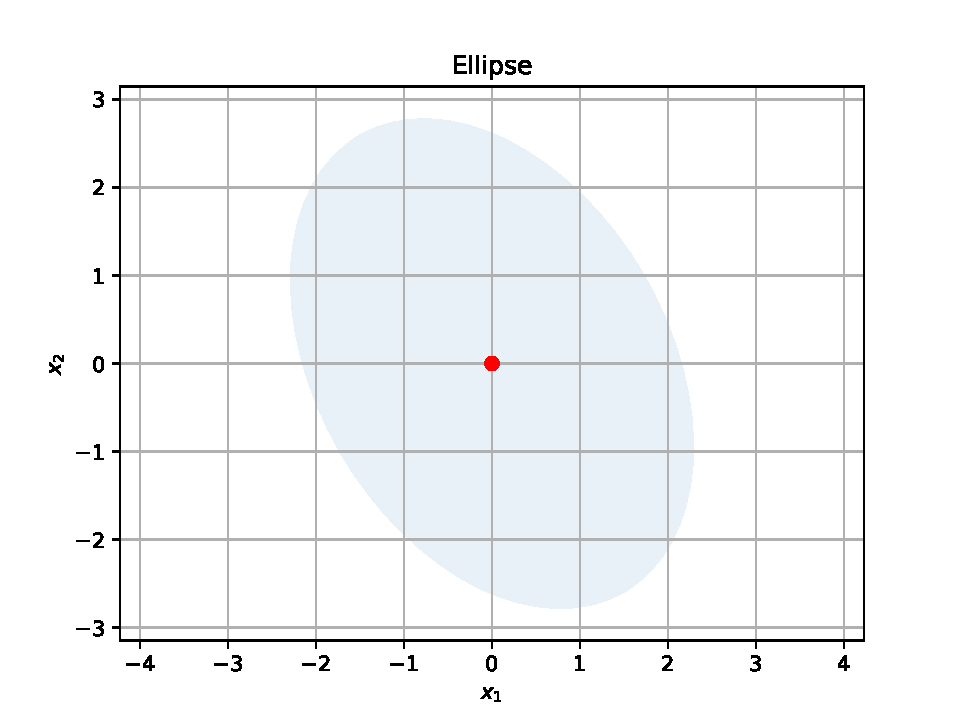
\includegraphics[scale = 0.5]{Ellipse.pdf}
    \caption{ p = 2 时 马氏距离的几何意义}
   \end{figure}

   如果是$p = 3$,即三维。其几何意义就是切不同的等高线。
   \[ \frac{y_{1}^{2} }{\lambda_{1}} + \frac{y_{2}^{2} }{\lambda_{2}} + \frac{y_{3}^{2} }{\lambda_{3}} = constant \]

   二维高斯分布经常用椭圆等高线表达。
   
   \begin{myexample}[问题]
    什么样的矩阵可以写成这种形式?
    \[ \boldsymbol{\Omega  = U \Lambda U^{T} } \]
   \end{myexample}

   总结:
   \begin{align*}
        Summary: \quad \Delta & = {\left( \boldsymbol{x - \mu}  \right)}^{T} 
        \boldsymbol{\Omega^{-1}} \left( \boldsymbol{x - \mu}  \right)
      = \sum_{i = 1}^{p} y_{i}^{2} {\lambda_{i}}^{-1}  \\
      p(\boldsymbol{x}) & = \frac{1}{{2 \pi}^{\frac{p}{2}} \left| \Omega \right|^{\frac{1}{2}} }  exp\{ \Delta \}
   \end{align*}

   其中$ y_{i} = {\left( \boldsymbol{x - \mu}  \right)}^{T}   \boldsymbol{u_{i}}$,$  \boldsymbol{y} = \begin{pmatrix}
    y_1 \\
    y_2 \\
    \vdots\\
    y_p
\end{pmatrix}$






































 \begin{Matlab}{MATLAB Code}
  Euler method for the ODE model
  u'(x)=x^2+x-u, x in [0,1]
  Initial condition: u(0)=0 ;
  Exact solution: u(x)=-exp(-x)+x^2-x+1.
  clear all;  clf
  \end{Matlab}
  
  \centerline{Python Code}
  \vspace{3ex}
  
  \begin{Python}{Python Code}
  #PythonDraw.py
  import turtle as t
  \end{Python}

\end{document}